\documentclass[11pt]{beamer}

\usetheme{Darmstadt}

\usepackage{times}
\usefonttheme{structurebold}

\usepackage[english]{babel}
\usepackage{pgf,pgfarrows,pgfnodes,pgfautomata,pgfheaps}
\usepackage{amsmath,amssymb}
\usepackage[latin1]{inputenc}
\usepackage{multicol}

\input{slabbrev}

\title{Space time problems that we need to think about}

\author{Jim Ramsay, McGill University   \\
      National Center for Atmospheric Research \\
      24 October 2014}
\date{}

\begin{document}

%  --------------------------------------------------------------------

\begin{frame}

\maketitle

\end{frame}

%  --------------------------------------------------------------------

\begin{frame}

\frametitle{Overview}

\bi
  \item Climate change the demand for modelling space/tie data
  \item Assessing our current space/time modelling technology
  \bi
    \item Time series origins
    \item The Gaussian framework
    \item The coordinate box
  \ei
  \item Texture over space and time domains and its implications
  \item Simplicial meshes as examples of alternative coordinate systems
  \item Where we need to get over the next couple of decades
\ei

\end{frame}

%  --------------------------------------------------------------------

\begin{frame}

\frametitle{Climate change and mitigation}

\bi
  \item The prospects for averting climate change are not promising
  \item With these changes will come huge challenges to human populations
  \item These populations will demand action from governments
  \item Governments will turn to the sciences for help
  \item Scientists will gain new sources of data, and will ask the 
  statistical community for help
  \item Will we be ready?
\ei

\end{frame}

%  --------------------------------------------------------------------

\begin{frame}

\frametitle{A quick look at our space/time modelling toolbox}

\bi
  \item Reviews of recent stats texts aimed at climate science have been instructive
  \item Much as been achieved, and there is no need to be apologetic
  \item But it's clear that we are yet not ready to offer much of real value
  \item We begin by looking at the mathematical substructure employed by current space/time modelling technology.
 \ei

\end{frame}

%  --------------------------------------------------------------------

\begin{frame}

\begin{center}
\includegraphics[height=3in, width=4in]{figs/StorchZwiers.pdf}
\end{center}

\end{frame}

%  --------------------------------------------------------------------

\begin{frame}

\begin{center}
\includegraphics[height=3in, width=4in]{figs/CressieWikle.pdf}
\end{center}

\end{frame}

%  --------------------------------------------------------------------

\begin{frame}

\frametitle{A quick look at our space/time modelling toolbox}

\bi
  \item Reviews of recent stats texts aimed at climate science have been instructive
  \item Much as been achieved, and there is no need to be apologetic
  \item But it's clear that we are yet not ready to offer much of real value
  \item We begin by looking at the mathematical substructure employed by current space/time modelling technology.
 \ei

\end{frame}

%  --------------------------------------------------------------------

\begin{frame}

\begin{center}
\includegraphics[height=3in, width=4in]{figs/BoxJenkinsReinsel.pdf}
\end{center}

\end{frame}

%  --------------------------------------------------------------------


%  --------------------------------------------------------------------

\begin{frame}

\begin{center}
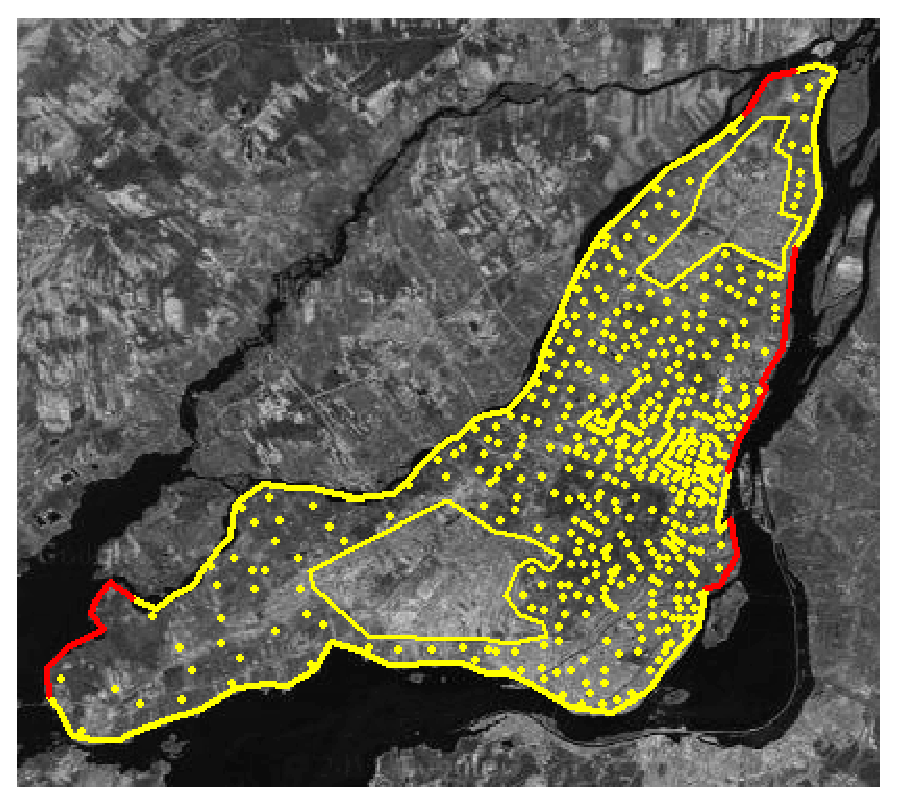
\includegraphics[height=3in, width=4in]{figs/Montreal_data_boundary_small.eps}
\end{center}

\end{frame}

%  --------------------------------------------------------------------

\begin{frame}

\frametitle{Census tract locations on the Island of Montreal}

\bi
  \item Yellow boundary points are locations of zero normal flow.
  \item Red boundary points are locations of zero level.
  \item Lower hole is Trudeau Airport.
  \item Upper hole is oil refinery and water treatment complex.
  \item This object is embedded in a two-dimensional locally Euclidean space.
  \item This space has no natural zero, is invariant under translations, and is therefore affine.
  \item There is no natural Cartesian coordinate system here, and consequently no vector space structure.
  \item We could compute principal components of point locations, but we would have to use a coordinate system to do.
\ei

\end{frame}

%  --------------------------------------------------------------------

\begin{frame}

\begin{center}
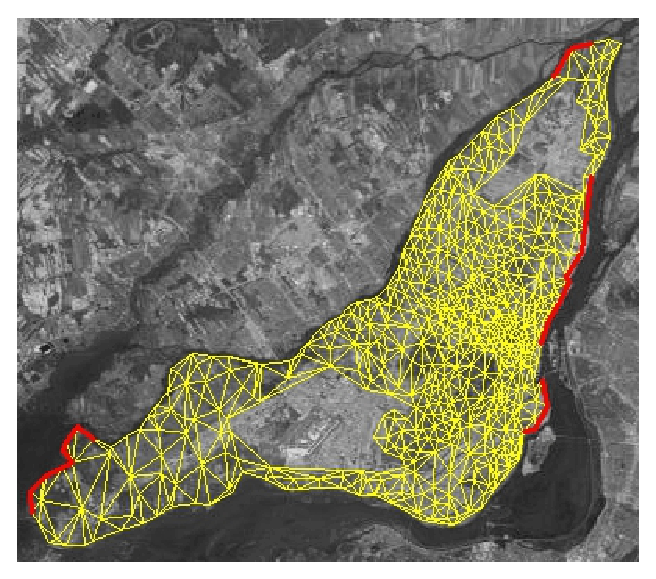
\includegraphics[height=3in, width=4in]{figs/fig_Montreal_triangulation_dirichlet_small.eps}
\end{center}

\end{frame}

%  --------------------------------------------------------------------

\begin{frame}

\frametitle{Census tract mesh on the Island of Montreal}

\bi
  \item Tract locations are vertices in a Delaunay triangulation.
  \item Now we have a two-level coordinate system:
  \bi
    \item Edges connect vertices
    \item Barycentric coordinates navigate us within triangles
  \ei
  \item We need to learn how to do data analysis with multi-level coordinate systems.
\ei

\end{frame}

%  --------------------------------------------------------------------

\begin{frame}

\begin{center}
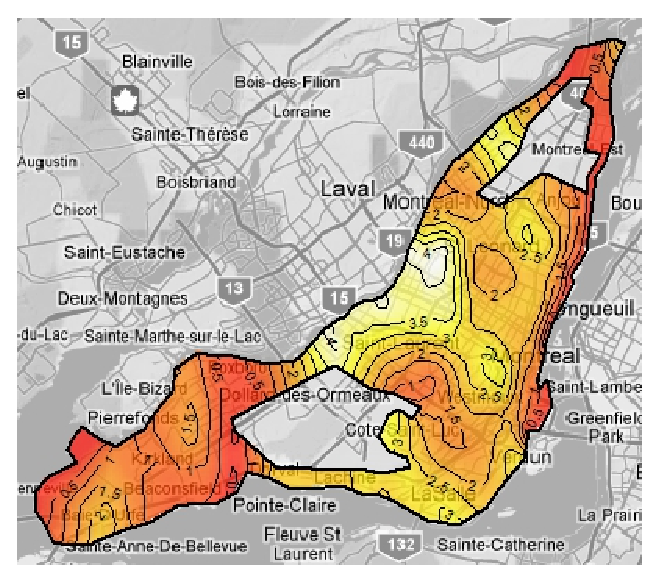
\includegraphics[height=3in, width=4in]{figs/fig_Montreal_results_dirichlet_small_ter.eps}
\end{center}

\end{frame}

%  --------------------------------------------------------------------

\begin{frame}

\frametitle{Smoothed annual income over the Island of Montreal}

Smoothing algorithm described in Sangalli, L. M., Ramsay, J. O. and Ramsay, T. O. (2013) Spatial spline regression models. \emph{Journal of the Royal Statistical Society, Series B,} {\bf 75}, 681-703.

\end{frame}

\end{document}